\documentclass[a4paper,french]{paper}
\usepackage{../../_latex_assets/villemejane_iogs_ceti}

%Informations about this document 
%------------------------------------------
\def\module{Ingénierie Electronique pour le Traitement de l'Information}
\def\moduleAbrege{6N-047-SCI / IéTI}
\def\annee{}

\def\titre{TD 2 / Pilotage d'une source à diodes}
\author{Julien VILLEMEJANE}

\subtitle{TD 2}
\institution{LEnsE / Institut d'Optique Graduate School}

\title{\titre}
\begin{document} 
%Beginning First Page. 
%------------------------------------------
\enteteThematiqueObligatoire{}

%Beginning Content. 
%------------------------------------------
\vspace{-1cm}
%%%%%%%%%%%%%%%
\encadreTDExo{1 - Conversion de signaux courants}{

%%%%%%%%%%%%%%%%%%%%%%%%%%%%%%%%%%%%
\subsection*{Signal audio}

\begin{enumerate}
	\item Rappeler l'intervalle de fréquences des signaux audibles par l'être humain.
	\item Quelle est la fréquence minimale pour échantillonner correctement un signal audio ?

Les signaux audio "classiques" (CD audio par exemple) sont échantillonnés à une fréquence $F_{Eclassique} = 44.1\operatorname{kHz}$ et chaque échantillon est codé sur 16~bits. 

Les signaux HRA (Audio Haute Résolution) sont échantillonnés à une fréquence $F_{EHRA1} = 96\operatorname{kHz}$ ou $F_{EHRA2} = 192\operatorname{kHz}$ et chaque échantillon est codé sur 24~bits.

	\item Ces fréquences sont-elles bien choisies ?
	\item Combien de niveau logique différent y a-t-il pour chacune de ces normes ?

	\item Quelle quantité d'espace numérique (en octets) faut-il prévoir pour stocker une heure de données sonores :
	\begin{enumerate}
		\item au format "classique", stéréo ?
		\item au format HRA-192, en 5.1 ?
	\end{enumerate}
\end{enumerate}

%%%%%%%%%%%%%%%%%%%%%%%%%%%%%%%%%%%%
\subsection*{Signal vidéo}

On s'intéresse au capteur \textbf{CMV50000} de la société \textit{CMOSIS}, capteur 8K@30fps - au prix d'environ 3500\$ (juin 2018) dont la documentation est donnée en annexe.

\begin{enumerate}
	\item Quelle est la taille de l'image de ce capteur ? Combien cela fait-il de pixels ?
	\item Combien de convertisseurs analogique-numérique embarquent ce capteur ? Quelle est la résolution des ADC ?
	\item La vitesse de transfert donnée est-elle suffisante pour prendre des images en 8K (7680 x 4320 pixels) à 30 images/seconde ?
\end{enumerate}
}

\newpage
%%%%%%%%%%%%%%%%%%%%%%%%%%%%%%%%%%%%%%%%%%%%%%%%%%%%%%%%%%%%%%%%%%%%%%%%%%
\encadreTDExo{2 - Système numérique}{

Que peut-on dire des signaux suivants ?

\begin{center}
	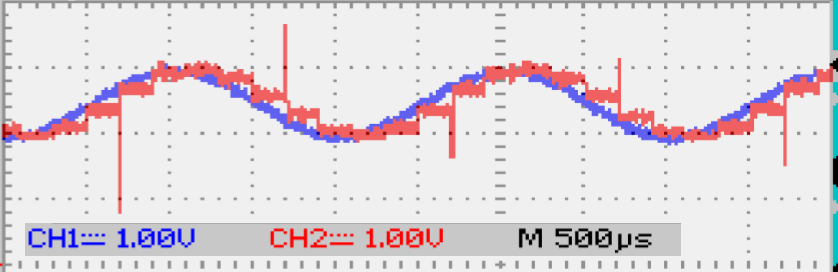
\includegraphics{images/TD/signal_num_1.png}\end{center}

\begin{center}
	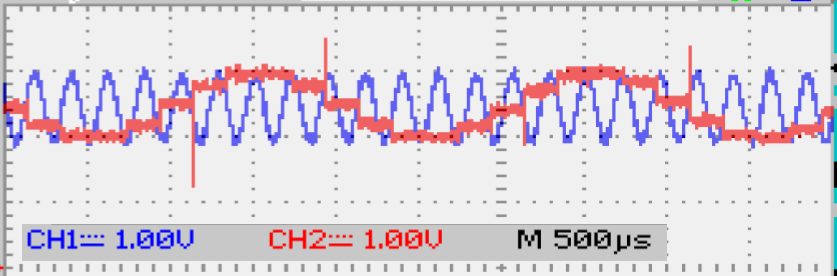
\includegraphics{images/TD/signal_num_2.png}\end{center}
}

%%%%%%%%%%%%%%%%%%%%%%%%%%%%%%%%%%%%%%%%%%%%%%%%%%%%%%%%%%%%%%%%%%%%%%%%%%
\encadreTDExo{3 - Entrées/Sorties Numériques}{


On s'intéresse à présent à 2 convertisseurs analogiques-numériques différents, dont une partie des documentations techniques sont données en annexe :
\begin{itemize}
	\item \textbf{TLC548} de \textit{Texas Instruments} (environ 3\$ - juin 2018)
	\item \textbf{AD9230} de \textit{Analog Devices} (environ 80\$ - juin 2018)
\end{itemize}

\begin{enumerate}
	\item A partir de ces deux documentations, remplir le tableau suivant :

\begin{tabular}{|c|p{3cm}|p{3cm}|}
\hline 
 & TLC548 & AD9230 \\ 
\hline 
Type de sortie &  &  \\ 
\hline 
$F_{Emax}$ &  &  \\ 
\hline 
Résolution &  &  \\ 
\hline 
Alimentation &  &  \\ 
\hline 
\end{tabular} 
	
	\item A l'aide de la documentation technique du \textbf{TLC548}, 
	\begin{enumerate}
		\item Expliquer à quoi correspondent les différents éléments du \textbf{diagramme fonctionnel} donnée en page 2.
		\item Expliquer l'opération de conversion et de récupération des données à partir de la \textbf{séquence} donnée en page 3.
		\item Combien de temps faut-il entre chaque conversion (pour $F_{CLOCK} = 2.048\operatorname{MHz}$ ?
	\end{enumerate}
	
\end{enumerate}
}

%%%%%%%%%%%%%%%%%%%%%%%%%%%%%%%%%%%%%%%%%%%%%%%%%%%%%%%%%%%%%%%%%%%%%%%%%%
\encadreTDExo{4 - Convertisseur R-2R}{

%%%%%%%%%%%%%%%%%%%%%%%%%%%%%%%%%%%%
\subsection*{Montage R-2R}

On s'intéresse à ce montage :

\begin{center}
	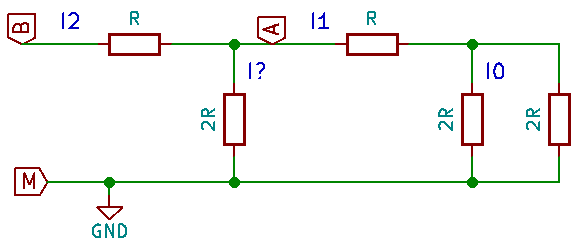
\includegraphics{images/TD/convAN_R2R_a.png}\end{center}


\begin{enumerate}
	\item Que vaut le courant $I_1$ en fonction du courant $I_0$ (courant passant par la résistance $2R$ ?
	\item Que vaut le courant $I_2$ en fonction du courant $I_0$ (courant passant par la résistance $2R$ ?	
\end{enumerate}

%%%%%%%%%%%%%%%%%%%%%%%%%%%%%%%%%%%%
\subsection*{Montage complet}

On s'intéresse à présent au montage suivant : 

\begin{center}
	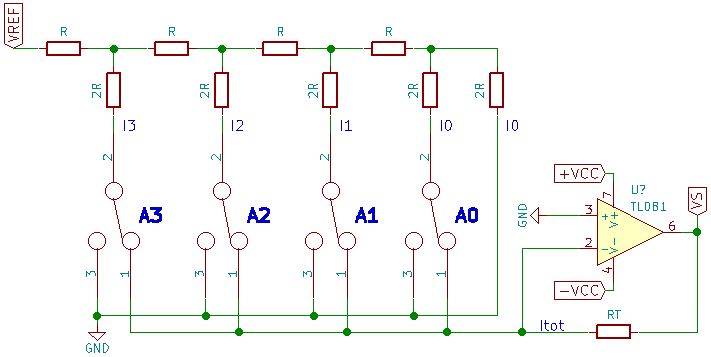
\includegraphics{images/TD/convAN_R2R_b.png}\end{center}

On supposera que lorsque $A_i = 0$, l'interrupteur $i$ est en position 3 et que lorsque $A_i = 1$, l'interrupteur $i$ est en position 1.

\begin{enumerate}
	\item Quel est le type de montage autour de l'ALI ?
	\item En quoi la structure vue précédemment peut nous aider ?
	\item Que vaut alors le courant $I_{tot}$ dans la contre-réaction de l'ALI en fonction des courants $I_i$ ?	
	\item Que vaut alors le courant $I_{tot}$ dans la contre-réaction de l'ALI en fonction du courant $I0i$ et des valeurs des $A_i$ ?

\end{enumerate}
}


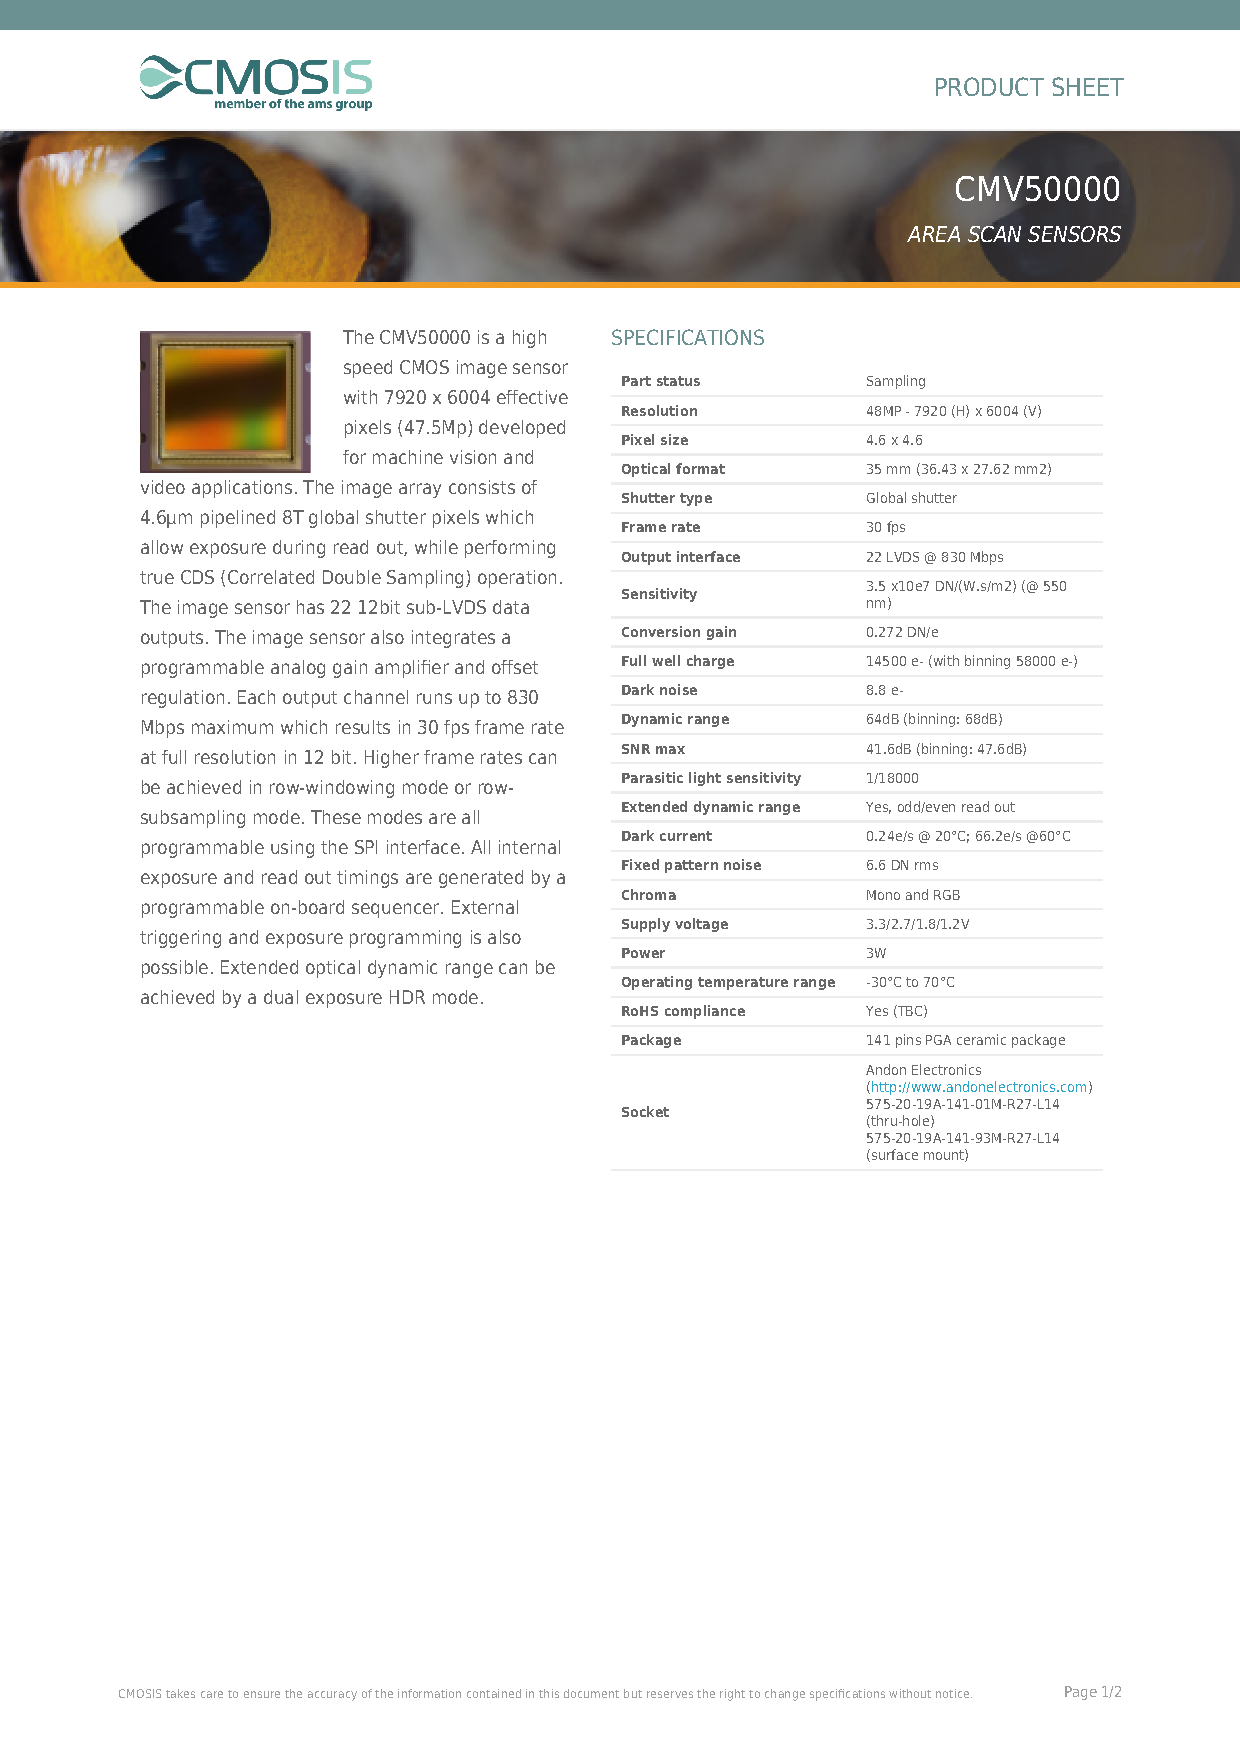
\includepdf[pages=-]{docs/CMOSIS_CMV5000.pdf}
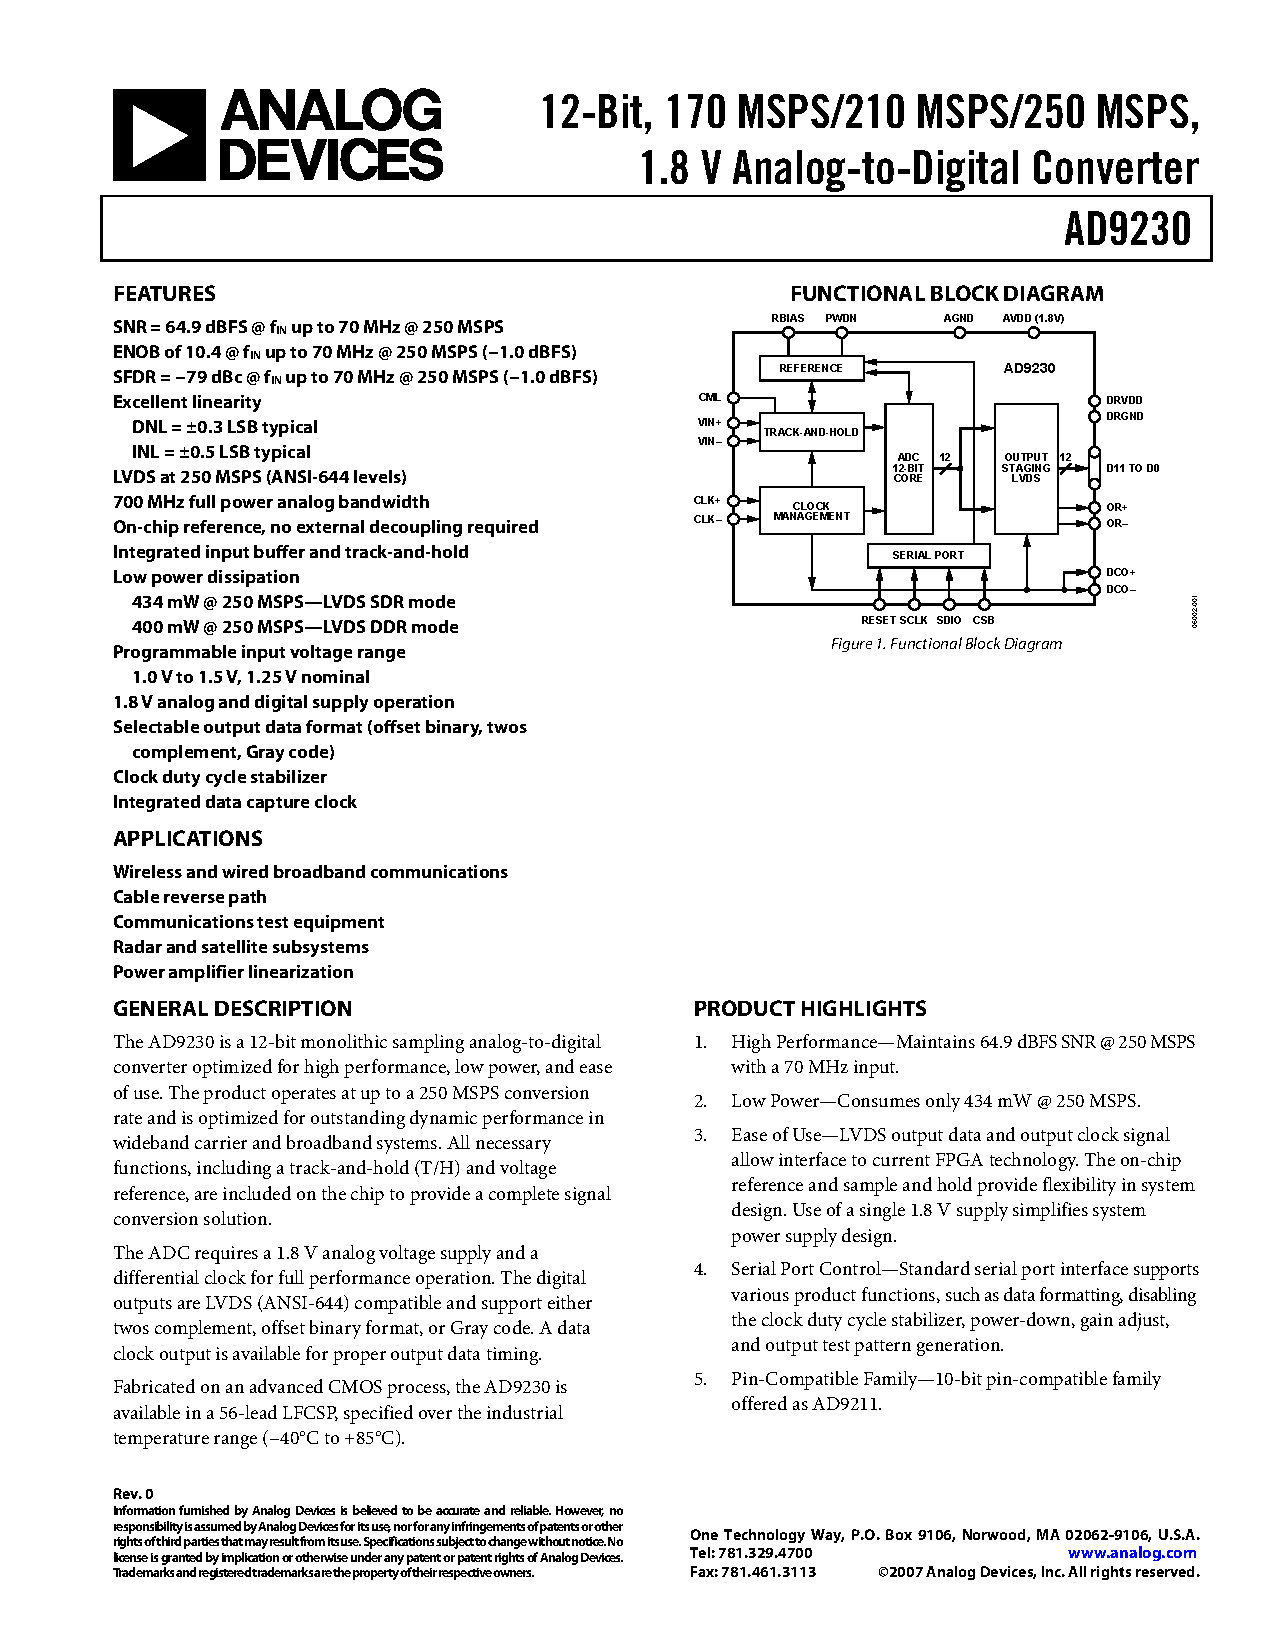
\includepdf[pages=1]{docs/AD9230_ADC_12bits.pdf}
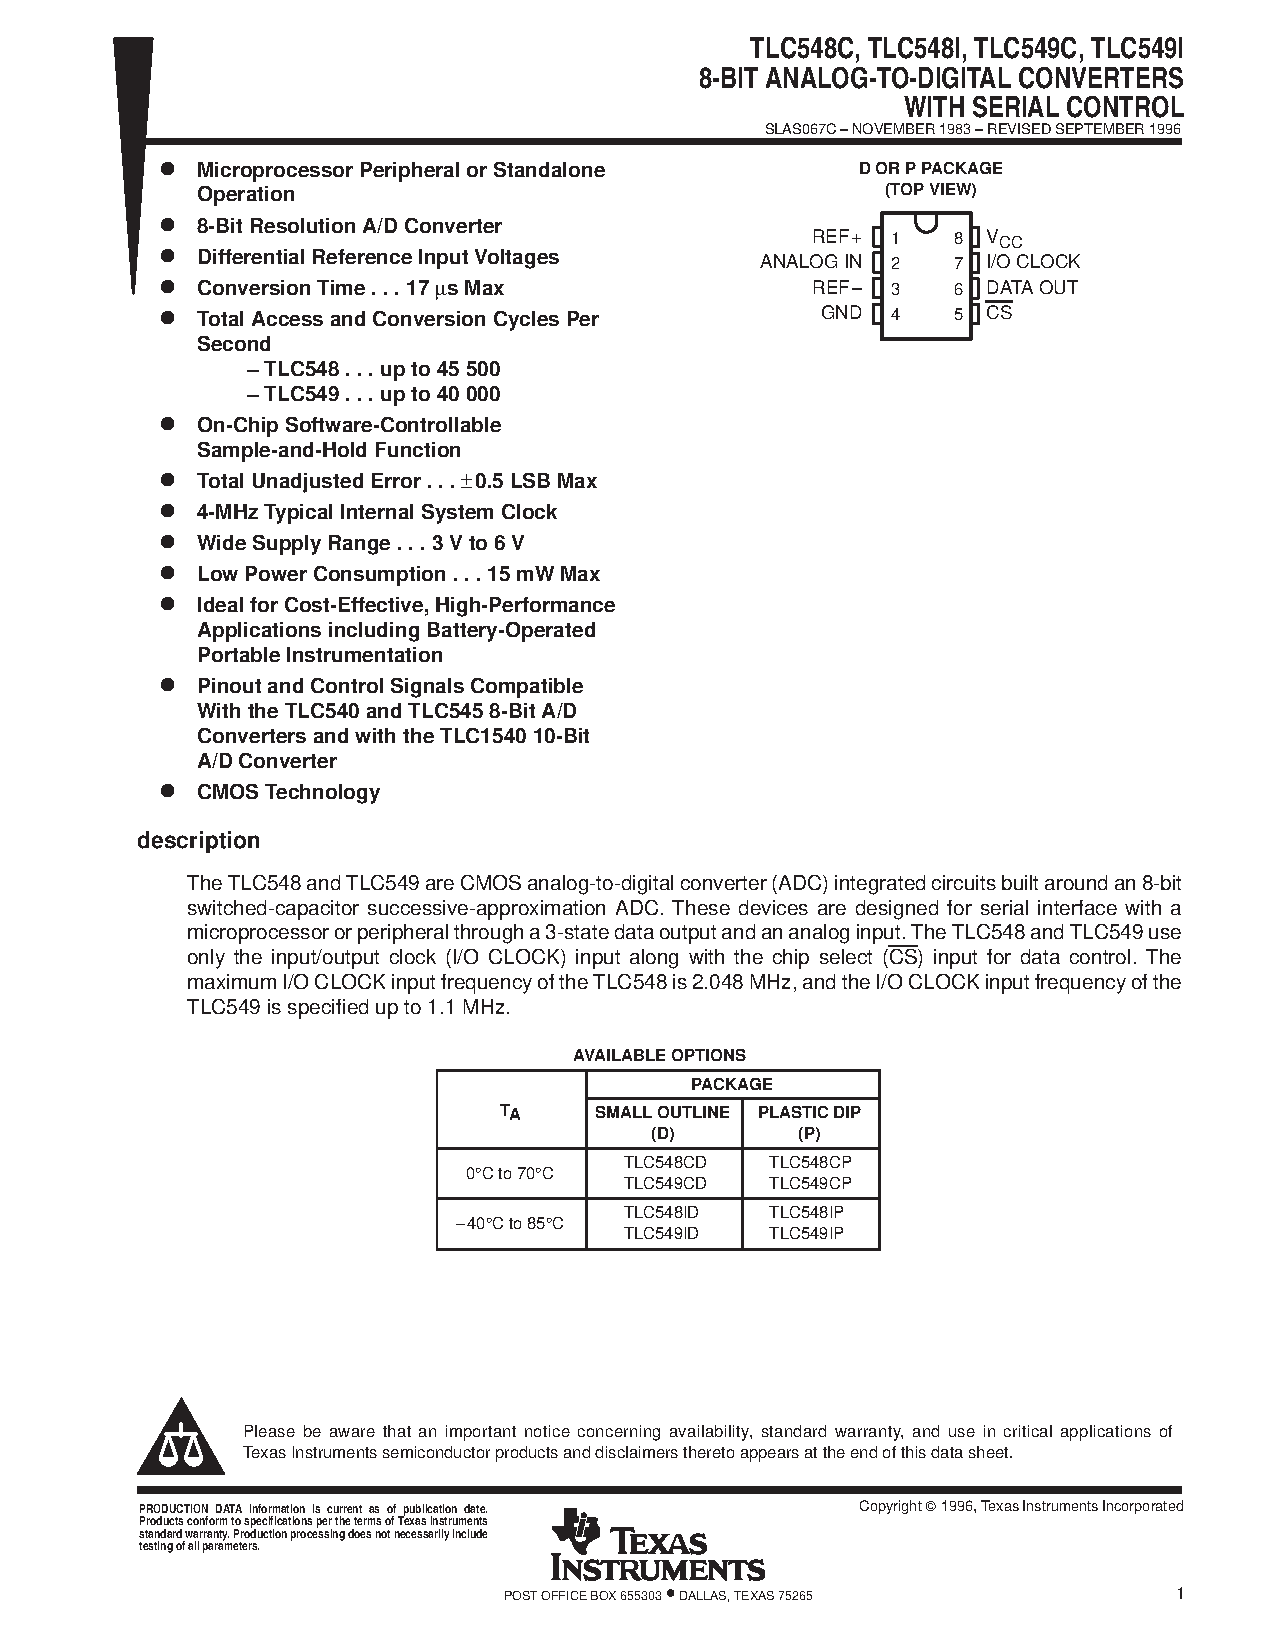
\includepdf[pages=-]{docs/TLC548_ADC_8bits.pdf}

\end {document}